\section{Variational Inference for non-Markovian Forward Processes}
\label{sec:variational}

Because the generative model approximates the reverse of the inference process, we need to rethink the inference process in order to reduce the number of iterations required by the generative model.
Our key observation is that the DDPM objective in the form of $L_\gamma$ only depends on the marginals\footnote{We slightly abuse this term (as well as joints) when only conditioned on $\bm{x}_0$.} $q(\bm{x}_t | \bm{x}_0)$, but not directly on the joint $q(\bm{x}_{1:T} | \bm{x}_{0})$. Since there are many inference distributions (joints) with the same marginals, we 
explore 
alternative
inference processes that are non-Markovian, which leads
to new generative processes (\Figref{fig:diffusion}, right). 
These non-Markovian inference process lead to the same surrogate objective function as DDPM, as we will show below.
In Appendix~\ref{app:discrete}, we show that the non-Markovian perspective also applies beyond the Gaussian case.

\subsection{Non-Markovian forward processes} 
Let us consider a family $\gQ$ of inference distributions, %
indexed by a real vector $\sigma \in \R_{\geq 0}^{T}$:
\begin{gather}
    q_\sigma(\bm{x}_{1:T} | \bm{x}_0) := q_\sigma(\bm{x}_T | \bm{x}_0) \prod_{t=2}^{T} q_\sigma(\bm{x}_{t-1} | \bm{x}_{t}, \bm{x}_0) \label{eq:diff-new}
\end{gather}
where $q_\sigma(\bm{x}_{T} | \bm{x}_0) = \mathcal{N}(\sqrt{\alpha_T} \bm{x}_0, (1 - \alpha_T) \bm{I})$ and for all $t > 1$,
\begin{gather} 
   q_\sigma(\bm{x}_{t-1} | \bm{x}_t, \bm{x}_0) = \mathcal{N}\left(\sqrt{\alpha_{t-1}} \bm{x}_{0} + \sqrt{1 - \alpha_{t-1} - \sigma^2_t} \cdot {\frac{\bm{x}_{t}  - \sqrt{\alpha_{t}} \bm{x}_0}{\sqrt{1 - \alpha_{t}}}}, \sigma_t^2 \bm{I} \right). \label{eq:reversed-close-form}
\end{gather}
The mean function is chosen to order to ensure that $q_\sigma(\bm{x}_{t} | \bm{x}_0) = \mathcal{N}(\sqrt{\alpha_t} \bm{x}_0, (1 - \alpha_t) \bm{I})$ for all $t$ 
(see Lemma~\ref{lemma:reverse-process-consistency} of Appendix~\ref{app:proofs}), so that it defines a joint inference distribution that matches the ``marginals'' as desired. %
The forward process\footnote{We overload the term ``forward process'' for cases where the inference model is not a diffusion.} can be derived from Bayes' rule:
\begin{align}
    q_\sigma(\bm{x}_{t} | \bm{x}_{t-1}, \bm{x}_0) = \frac{q_\sigma(\bm{x}_{t-1} | \bm{x}_{t}, \bm{x}_0) q_\sigma(\bm{x}_{t} | \bm{x}_0)}{q_\sigma(\bm{x}_{t-1} | \bm{x}_0)}, \label{eq:bayes-rule}
\end{align}
which is %
also Gaussian (although we do not use this fact for the remainder of this paper).
Unlike the diffusion process in \eqref{eq:diff-ho}, %
the forward process here is no longer Markovian, since each $\bm{x}_t$ could depend on both $\bm{x}_{t-1}$ and $\bm{x}_0$. The magnitude of $\sigma$ controls the how stochastic the forward process is; when $\sigma \to \bm{0}$, %
we reach an extreme case where as long as we observe $\bm{x}_0$ and $\bm{x}_t$ for some $t$, then $\bm{x}_{t-1}$ become known and fixed. %



\subsection{Generative process and unified variational inference objective}


Next, we define a trainable generative process $p_\theta(\bm{x}_{0:T})$ where each $p_{\theta}^{(t)}(\bm{x}_{t-1} | \bm{x}_t)$ %
 leverages knowledge of $q_\sigma(\bm{x}_{t-1} | \bm{x}_{t}, \bm{x}_0)$. %
Intuitively, given a noisy observation $\bm{x}_t$, we first make a prediction\footnote{Learning a distribution over the predictions is also possible, but empirically we found little benefits of it.} of the corresponding $\bm{x}_0$, 
and then use it to obtain a sample $\bm{x}_{t-1}$ through the reverse conditional distribution $q_\sigma(\bm{x}_{t-1} | \bm{x}_{t}, \bm{x}_0)$, which we have defined. %

For some $\bm{x}_0 \sim q(\bm{x}_0)$ and $\epsilon_t \sim \mathcal{N}(\bm{0}, \bm{I})$, 
$\bm{x}_t$ can be obtained using \eqref{eq:reparam_xt}. The model $\epsilon_\theta^{(t)}(\bm{x}_t)$ then attempts to predict $\epsilon_t$ from $\bm{x}_t$, without knowledge of $\bm{x}_0$.
By rewriting \eqref{eq:reparam_xt}, one can then predict the \textit{denoised observation}, which is a prediction of $\bm{x}_0$ given $\bm{x}_t$:
\begin{align}
    f_\theta^{(t)}(\bm{x}_t) := (\bm{x}_t - \sqrt{1 - \alpha_t} \cdot \epsilon_{\theta}^{(t)}(\bm{x}_t)) / \sqrt{\alpha_t}. \label{eq:x0-pred-def}
\end{align}
We can then define the generative process with a fixed prior $p_\theta(\bm{x}_T) = \mathcal{N}(\bm{0}, \bm{I})$ and
\begin{align}
    p_\theta^{(t)}(\bm{x}_{t-1} | \bm{x}_t) = \begin{cases}
    \mathcal{N}(f_\theta^{(1)}(\bm{x}_1), \sigma_1^2 \bm{I})  & \text{if} \ t = 1 \\
    q_\sigma(\bm{x}_{t-1} | \bm{x}_t, f_{\theta}^{(t)}(\bm{x}_t)) & \text{otherwise,}
    \end{cases} \label{eq:new-reverse}
\end{align}
where $q_\sigma(\bm{x}_{t-1} | \bm{x}_t, f_{\theta}^{(t)}(\bm{x}_t))$ is defined as in \eqref{eq:reversed-close-form} with $\bm{x}_0$ replaced by $f_{\theta}^{(t)}(\bm{x}_t)$. %
We add some Gaussian noise (with covariance $\sigma_1^2 \bm{I}$) for the case of $t = 1$ to ensure that the generative process is supported everywhere. 

We optimize $\theta$ via the following variational inference objective (which is a functional over $\epsilon_\theta$):
\begin{align}
   & J_\sigma(\epsilon_\theta) :=
   \bb{E}_{\bm{x}_{0:T} \sim q_\sigma(\bm{x}_{0:T})}[\log q_\sigma(\bm{x}_{1:T} | \bm{x}_0) - \log p_\theta(\bm{x}_{0:T})] \\
   = & \ \bb{E}_{\bm{x}_{0:T} \sim q_\sigma(\bm{x}_{0:T})} \left[\log q_\sigma(\bm{x}_T | \bm{x}_0) + \sum_{t=2}^{T} \log q_\sigma(\bm{x}_{t-1} | \bm{x}_t, \bm{x}_0) - \sum_{t=1}^{T} \log p_\theta^{(t)}(\bm{x}_{t-1} | \bm{x}_t) - \log p_\theta(\bm{x}_T) \right] \nonumber%
\end{align}
where we factorize $q_\sigma(\bm{x}_{1:T} | \bm{x}_0)$ according to \eqref{eq:diff-new} and $p_\theta(\bm{x}_{0:T})$ according to \eqref{eq:gen}.


From the definition of $J_\sigma$, it would appear that a different model has to be trained for every choice of $\sigma$, since it corresponds to a different variational objective (and a different generative process). %
However, $J_\sigma$ is equivalent to $L_\gamma$ for certain weights $\gamma$, as we show below.
\begin{restatable}{theorem}{unifiedklobj}
\label{thm:unifiedklobj}
For all $\sigma > \bm{0}$, there exists $\gamma \in \R_{> 0}^{T}$ and $C \in \R$, such that $J_\sigma = L_\gamma + C$.
\end{restatable}
The variational objective $L_\gamma$ is special in the sense that if parameters $\theta$ %
of the models $\epsilon_\theta^{(t)}$ %
are not shared across different $t$, then the optimal solution for $\epsilon_\theta$ will not depend on the weights $\gamma$ (as global optimum is achieved by separately maximizing each term in the sum). 
This property of $L_\gamma$ has two implications. %
On the one hand, this justified the use of $L_\vone$ as a surrogate objective function for the variational lower bound in DDPMs; on the other hand, since $J_\sigma$ is equivalent to some $L_\gamma$ from Theorem~\ref{thm:unifiedklobj}, the optimal solution of $J_\sigma$ is also the same as that of $L_\vone$. %
Therefore, if parameters are not shared across $t$ in the model $\epsilon_\theta$, then the $L_\vone$ objective used by \citet{ho2020denoising} can be used as a surrogate objective for the variational objective $J_\sigma$ as well. 




\section{Sampling from Generalized Generative Processes}\label{sec:sampling}
With $L_\vone$ as the objective, we are not only learning a generative process for the Markovian inference process considered in \citet{sohl-dickstein2015deep} and \citet{ho2020denoising}, but also generative processes for many non-Markovian forward processes parametrized by $\sigma$ %
that we have described. Therefore, we can essentially use pretrained DDPM models as the solutions to the new objectives, and focus on finding a generative process that is better at producing samples subject to our needs by changing $\sigma$. %
\subsection{Denoising Diffusion Implicit Models}
\label{sec:reverse-family}
From $p_\theta(\bm{x}_{1:T})$ in \eqref{eq:new-reverse}, one can generate a sample $\bm{x}_{t-1}$ from a sample $\bm{x}_{t}$ via:
\begin{align}
    \bm{x}_{t-1} & = \sqrt{\alpha_{t-1}} \underbrace{\left(\frac{\bm{x}_t - \sqrt{1 - \alpha_t} \epsilon_\theta^{(t)}(\bm{x}_t)}{\sqrt{\alpha_t}}\right)}_{\text{`` predicted } \bm{x}_0 \text{''}} + \underbrace{\sqrt{1 - \alpha_{t-1} - \sigma_t^2} \cdot \epsilon_\theta^{(t)}(\bm{x}_t)}_{\text{``direction pointing to } \bm{x}_t \text{''}} + \underbrace{\sigma_t \epsilon_t}_{\text{random noise}} \label{eq:sample-eq-gen}
\end{align}
where $\epsilon_t \sim \mathcal{N}(\bm{0}, \bm{I})$ is standard Gaussian noise independent of $\bm{x}_t$, and we define $\alpha_0 := 1$. Different choices of $\sigma$ values results in different generative processes, all while using the same model $\epsilon_\theta$, so re-training the model is unnecessary. When $\sigma_t = \sqrt{(1 - \alpha_{t-1}) / (1 - \alpha_t)} \sqrt{1 - \alpha_t / \alpha_{t-1}}$ for all $t$, the forward process becomes Markovian, and the generative process becomes a DDPM.

We note another special case when $\sigma_t = 0$ for all $t$\footnote{Although this case is not covered in Theorem~\ref{thm:unifiedklobj}, we can always approximate it by making $\sigma_t$ very small.}; the forward process becomes deterministic given $\bm{x}_{t-1}$ and $\bm{x}_0$, except for $t = 1$; in the generative process, the coefficient before the random noise $\epsilon_t$ becomes zero. %
The resulting model becomes an implicit probabilistic model~\citep{mohamed2016learning}, where samples are generated from latent variables with a fixed procedure (from $\bm{x}_T$ to $\bm{x}_0$). We name this the \textit{denoising diffusion implicit model} (DDIM, pronounced \textipa{/d:Im/}), because it is an implicit probabilistic model trained with the DDPM objective (despite the forward process no longer being a diffusion). 





\subsection{Accelerated generation processes}
\label{sec:acceleration}
In the previous sections, the generative process is considered as the approximation to the reverse process; since of the forward process has $T$ steps, the generative process is also forced to sample $T$ steps. However, as the denoising objective $L_\vone$ does not depend on the specific forward procedure as long as $q_\sigma(\bm{x}_{t} | \bm{x}_0)$ is fixed, we may also consider forward processes with lengths smaller than $T$, which accelerates the corresponding generative processes without having to train a different model.


\begin{figure}
\centering
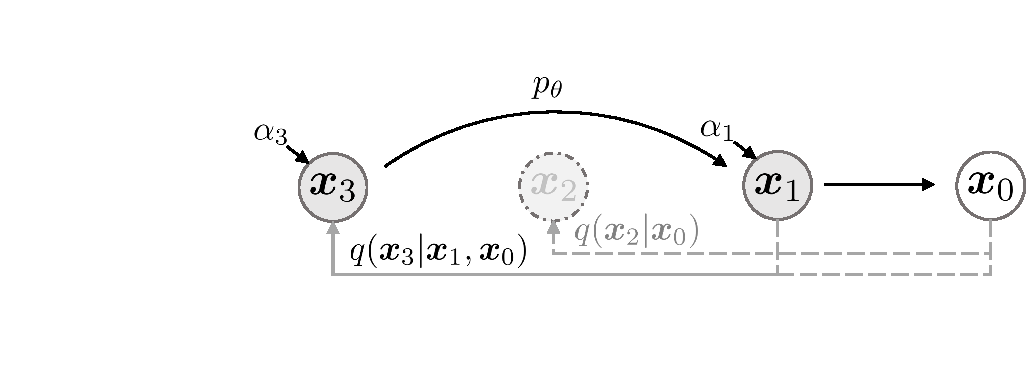
\includegraphics[width=0.5\textwidth]{figures/diffusion-figure-acc.pdf}
\captionof{figure}{Graphical model for accelerated generation, where $\tau = [1, 3]$.}
\label{fig:diffusion-figure-acc}
\end{figure}

Let us consider the forward process as defined not on all the latent variables $\bm{x}_{1:T}$, but on a subset $\{\bm{x}_{\tau_1}, \ldots, \bm{x}_{\tau_S}\}$, where $\tau$ is an increasing sub-sequence of $[1, \ldots, T]$ of length $S$. 
In particular, we define the sequential forward process over $\bm{x}_{\tau_1}, \ldots, \bm{x}_{\tau_S}$ such that $q(\bm{x}_{\tau_i} | \bm{x}_0) = \mathcal{N}(\sqrt{\alpha_{\tau_i}} \bm{x}_0, (1 - \alpha_{\tau_i}) \bm{I})$ matches the ``marginals'' (see \Figref{fig:diffusion-figure-acc} for an illustration).
The generative process now samples latent variables according to $\text{reversed}(\tau)$, which we term \textit{(sampling) trajectory}. When the length of the sampling trajectory is much smaller than $T$, we may achieve
significant increases in computational efficiency due to the iterative nature of the sampling process. 

Using a similar argument as in Section~\ref{sec:variational}, we can justify using the model trained with the $L_\vone$ objective, so no changes are needed in training. We show that only slight changes to the updates in \eqref{eq:sample-eq-gen} are needed to obtain the new, faster generative processes, which applies to DDPM, DDIM, as well as all generative processes considered in \eqref{eq:new-reverse}.
We include these details in Appendix~\ref{app:acceleration}.







In principle, this means that we can train a model with an arbitrary number of forward steps but only sample from some of them in the generative process. Therefore, the trained model could consider many more steps than what is considered in \citep{ho2020denoising} or even a continuous time variable $t$ \citep{chen2020wavegrad}. We leave empirical investigations of this aspect as future work.


\subsection{Relevance to Neural ODEs}
Moreover, we can rewrite the DDIM iterate according to \eqref{eq:sample-eq-gen}, and its similarity to Euler integration for solving ordinary differential equations (ODEs) becomes more apparent:
\begin{align}
    \frac{\bm{x}_{t-\Delta t}}{\sqrt{\alpha_{t-\Delta t}}}  = \frac{\bm{x}_t}{\sqrt{\alpha_t}}  + \left(\sqrt{\frac{1 - \alpha_{t-\Delta t}}{\alpha_{t-\Delta t}}} - \sqrt{\frac{1 - \alpha_{t}}{\alpha_t}}\right) \epsilon_\theta^{(t)}(\bm{x}_t) \label{eq:ddim-euler}
\end{align}
To derive the corresponding ODE, we can reparameterize $(\sqrt{1 - \alpha} / \sqrt{\alpha})$ with $\sigma$ and $(\bm{x} / \sqrt{\alpha})$ with $\bar{\bm{x}}$. In the continuous case, $\sigma$ and $\bm{x}$ are functions of $t$, where $\sigma: \bb{R}_{\geq 0} \to \bb{R}_{\geq 0}$ is continous, increasing with $\sigma(0) = 0$.
\Eqref{eq:ddim-euler} with can be treated as a Euler method over the following ODE:
\begin{align}
   \diff \bar{\bm{x}}(t) = \epsilon_\theta^{(t)}\left(\frac{\bar{\bm{x}}(t)}{\sqrt{\sigma^2 + 1}}\right) \diff \sigma(t) \label{eq:ddim-ode},
\end{align}
where the initial conditions is $\bm{x}(T) \sim \mathcal{N}(0, \sigma(T))$ for a very large $\sigma(T)$ (which corresponds to the case of $\alpha \approx 0$). This suggests that with enough discretization steps, the we can also reverse the generation process (going from $t = 0$ to $T$), which encodes $\bm{x}_0$ to $\bm{x}_T$ and simulates the reverse of the ODE in \eqref{eq:ddim-ode}. This suggests that unlike DDPM, we can use DDIM to obtain encodings of the observations (as the form of $\bm{x}_T$), which might be useful for other downstream applications that requires latent representations of a model.

In a concurrent work, \citep{song2020score} proposed a ``probability flow ODE'' that aims to recover the marginal densities of a stochastic differential equation (SDE) based on scores, from which a similar sampling schedule can be obtained. Here, we state that the our ODE is equivalent to a special case of theirs (which corresponds to a continuous-time analog of DDPM).
\begin{restatable}{proposition}{equivalence}
The ODE in \eqref{eq:ddim-ode} with the optimal model $\epsilon_\theta^{(t)}$ has an equivalent probability flow ODE corresponding to the ``Variance-Exploding'' SDE in \citet{song2020score}.
\end{restatable}
We include the proof in Appendix~\ref{app:proofs}. While the ODEs are equivalent, the sampling procedures are not, since the Euler method for the probability flow ODE will make the following update:
\begin{align}
    \frac{\bm{x}_{t-\Delta t}}{\sqrt{\alpha_{t-\Delta t}}}  = \frac{\bm{x}_t}{\sqrt{\alpha_t}}  + \frac{1}{2}\left(\frac{1 - \alpha_{t-\Delta t}}{\alpha_{t-\Delta t}} - \frac{1 - \alpha_{t}}{\alpha_t}\right) \cdot \sqrt{\frac{\alpha_t}{1 - \alpha_t}} \cdot \epsilon_\theta^{(t)}(\bm{x}_t) \label{eq:pf-euler}
\end{align}
which is equivalent to ours if $\alpha_t$ and $\alpha_{t-\Delta t}$ are close enough. In fewer sampling steps, however, these choices will make a difference; we take Euler steps with respect to $\diff \sigma(t)$ (which depends less directly on the scaling of ``time'' $t$) whereas \citet{song2020score} take Euler steps with respect to $\diff t$.



